\section{Evaluation of Tools and Techniques}
\label{sec:tools}

A number of different tools were used in the day to day running of the project.
These tools were used to ease the collaboration between members by ensuring that everyone knew
what they were supposed to be doing and how to share it with the others.

\subsection{Source Control: Git}

Source control systems are an essential tool for software projects, especially those
with multiple developers. Using source control to easily track the changes to source
code is helpful because, as McConnell explains, having a history of changes helps a
developer to identify the origin of bugs quickly.\citepage{mcconnell2004}{page 667}

The Git source control system\sidenote{\url{http://git-scm.com/}} was chosen for this project.
Git was chosen for a number of reasons. Firstly, it has a lightweight branching model which
allows for quick creation of new development branches for experimental features independent of
any other development. Chacon notes this as Git's ``killer feature''.\citepage{chacon2009}{page 38}
Another reason for choosing Git is its distributed nature. Every user has a full clone of the
entire repository that can act as a replacement for any other instance of the repository; this means
that there is no single, centralised point of failure.

A centralised master repository was hosted on Github, a popular code host.\sidenote{\url{https://github.com/}}
This made it easier for team members to share their changes to the code base. Once a change has been made
it can be `pushed' to the Github repository; other team members can then `pull' it to their local
repositories.

Git was an ideal source control system for the project. Not only does it allow the users to see
the entire history of changes made to the project it makes collaborative development between
multiple team members incredibly easy. Instead of having to resolve conflicting changes to files
it is possible to use the built in merge tool to combine the work of two or more people on the
same set of files with minimal effort. Git is recommended for all future development projects.

\subsection{Tracking and Managing Releases: Trello}

\begin{marginfigure}
	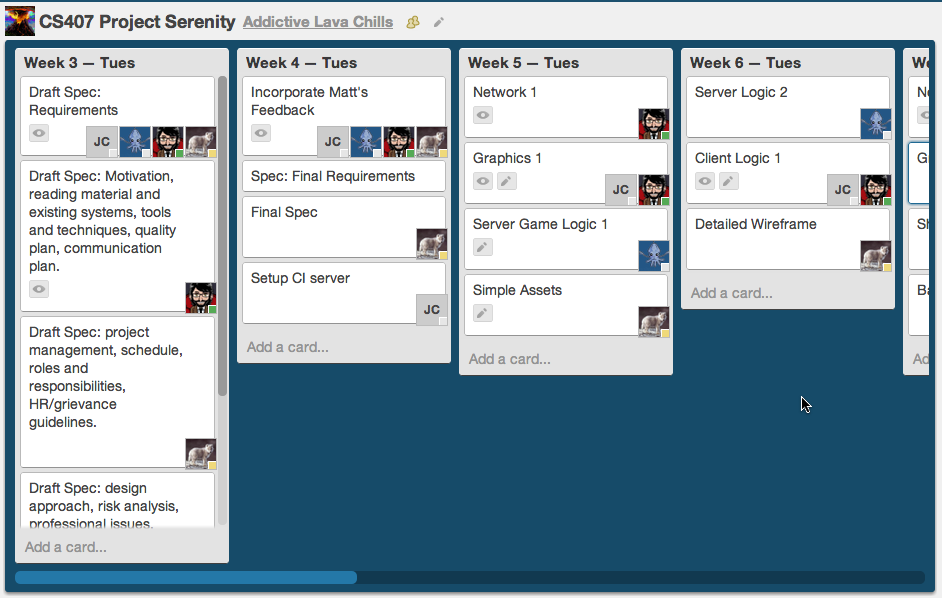
\includegraphics[width=6cm]{res/trello.png}
	\caption[Trello]{Project Serenity's Trello page}
	\label{fig:trello}
\end{marginfigure}

Trello is a modern, online take of an age old concept --- a wall of post-its. Trello allows for overall planning of tasks and communication between members in a highly dynamic, fluid way. Cards are arranged into a list-of lists, each list being some kind of functional decomposition or `stovepipe'. Trello has been used in the project to track the requirements for each weeks releases, but still allowing rapid changes to be made and communicated.

Trello acted as a useful reference to the current state of the project: what tasks are planned and who is doing them.
It is a good tool for keeping a small group of people organised, but requires careful management to keep it
up to date and useful.

\subsection{Bug Tracking: Github Issues}

Trello does not entirely alleviate the need for a full bug tracker. When working of development of
individual features and components it was necessary to have a method of tracking more transient issues
and tasks. The initial plan was to use the service provided by Fogbugz, a stand alone bug tracking
web application. However, in the end the Issues feature built into Github hosted repositories was
used. This was decided because it reduced the number of third party services that were relied upon
and it provided better integration with the hosted repository itself. Although it is much more minimal
than Fogbuz, it provided enough features, such as milestones, labels, email notifications, and
issue assignment, for this project.

An issue tracker was very useful for noting down smaller tasks and bugs that cannot be fixed immediately,
but must not be accidentally forgotten about. If a project is using Github to host code then the
Issues component is recommended if only simple issue tracking features are required. However, for
more complex requirements a more fully featured service may be a better option.

\subsection{Backups}

Backups of the source code and other project assets are essential. In the event of a
disaster, such as losing a computer to a fire, it must be possible to recreate the
entire project in its latest state quickly and without any repetition of work.\citepage{mcconnell2004}{page 669}
The use of Git and Github for source control made it simple to ensure that all
source code was located on multiple computers. By `pushing' commits to the Github
repository all code was stored in the cloud. When other team members `pulled' the code
later on it was then mirrored on their computers as well. Extra precautions were taken
by also `pushing' the Git repository to private servers owned by the team members.
Also, the free service provided by Dropbox\sidenote{\url{https://www.dropbox.com/}}
was used to share and backup any other files, such as assets and planning notes.

Fortunately a situation which required recovery from backups was never encountered,
but the strategies put it place should have been more than adequate if the need ever
arises in the future. Since the main backup strategy was part of normal development
workflow it was impossible to forget to implement it. However, it does have to be ensured that
all members are sharing their changes as frequently as possible (even if a feature is
not fully finished) to prevent any work in progress from being lost in case an individual's
computer dies. The extension to this core backup strategy, storing the repositories
on other personal servers, was easy because of Git's feature set which was designed
to be distributed in nature and so allows tracking and updating of multiple remote repositories.

\subsection{Continuous Integration: Jenkins}

Section~\ref{sec:testing} introduced the idea of continuous integration as a method
of regularly running the test suite and performing a full build of the software.
The Jenkins continuous integration server\sidenote{\url{http://jenkins-ci.org/}}
was used for this project. Jenkins was chosen because it is a widely used open
source project.\sidenote{\url{http://stats.jenkins-ci.org/jenkins-stats/}}
Jenkins also works well with projects hosted on Github because of its Github plugin\sidenote{\url{https://wiki.jenkins-ci.org/display/JENKINS/GitHub+Plugin}}
and Github's Jenkins specific post-receive hook.

Although Jenkins does not have a very good user interface it suited the needs of
this project. It was a good tool for running a test suite with every change to the
code base and ensuring that the game would build correctly. Email notifications on failure
were useful, but also relatively noisy at times. Continuous integration is probably
more useful for more mature projects that need to ensure that changes do not introduce
any regressions than it is for a project in the early stages of development when a lot
of features are not fully working.
